\documentclass[a4paper,11pt,dvipdfmx]{ujarticle}
% パッケージ
\usepackage{graphicx}
\usepackage{url}
% レイアウト指定を記述したファイルの読み込み
\input{layout}

% タイトルと氏名を変更せよ.
\title{日本におけるデジタル化の状況}
\author{G585102025 池森 皇哉}

\begin{document}

\maketitle %ここにタイトルが入る

% ここから本文
\section{デジタル競争力ランキング}
% を使う
国際経営開発研究所(IMD)の調査\cite{imd}によると、日本のデジタル競争力のランキングは図\ref{fig:ランキング}がが示すように、調査対象の64カ国中、総合で28位、知識分野で25位となっている
\begin{figure}[htbp]
    \centering
    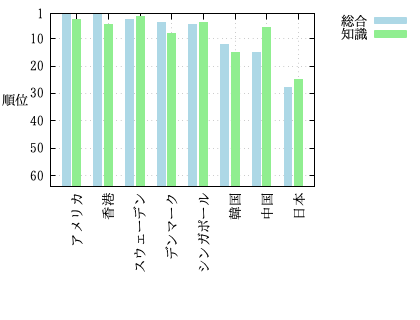
\includegraphics[width=0.7\linewidth]{fig31.png}
    \caption{デジタル競争力ランキング(64カ国中)}\label{fig:ランキング}
\end{figure}


\section{ブロードバンドの整備状況}

OECDによるブロードバンド回線の普及いかんする調査\cite{oecd}によると、表\ref{fig:表の挿入}に示すように、日本における100人あたりの光ファイバー回線の加入者数は29.0で、韓国、スウェーデン、ノルウェーの続いて第4位になっている。
\begin{table}[htbp]
     \centering
     \caption{光ファイバー回線の加入者人数(100人あたり)}\label{fig:表の挿入}
     \begin{tabular}{|c|l|r|}
         \hline
          順位 & 国名 & 加入者数 \\
          \hline
          1位 & 韓国 & 38.2 \\
          \hline
         2位 & スウェーデン & 31.9 \\
         \hline
         3位 & ノルウェー & 29.5 \\
         \hline
         4位 & 日本 & 29 \\
         \hline
         5位 & アイスランド & 28.8 \\
         \hline
         6位 & スペイン & 27.3 \\
         \hline
         7位 & ポルトガル & 25.1 \\
         \hline
         8位 & ニュージーランド & 23.6 \\
         \hline
         9位 & リトアニア & 22.3 \\
         \hline
         10位 & フランス & 1.2 \\
          \hline
    \end{tabular}
\end{table}


\section{考察}
\begin{itemize}
    \item 日本のデジタル競争力は低い.国際経営開発研究所(IMD)のランキングでは、日本は総合順位・知識順位ともに下位(64カ国中で50位前後)に位置しており、他の先進国と比べてかなり低いことがわかる。
    \item ブロードバンド普及率は比較的高い.OECDのデータによると、日本の光ファイバー回線の加入者数は100人あたり29.0人で4位となっており、通信インフラ自体は整っている。
    \item インフラ整備と活用度のギャップ.ブロードバンド環境が整っている一方で、デジタル競争力の低さが目立つことから、単にインフラがあるだけではデジタル化は進まないことが示唆される。
\end{itemize}

    

 






%  図番号の参照: \ref{}
% を使う
% 文献データベースのキーワードは oecd と imd
% になっている.

% 図の挿入
% \includegraphics{}
% を
% \begin{figure}[htbp]
% \end{figure}
% で囲み
% \caption{}
% で図のタイトルを入れる.
% \label{}
% を使って図番号が参照できるようにする
% また,
% \centering
% で図が中央に来るようにする

% ーーー
% 節見出し(2)

% 本文(2)

% 表の挿入
% \begin{tabular}
% \end{tabular}    
% による表の記述を 
% \begin{table}[htbp]
% \end{table}
% で囲み
% \caption{}
% で表のタイトルを入れる.
% \label{}
% を使って表番号が参照できるようにする
% また,
% \centering
% で表が中央に来るようにする

% ーーー
% 見出し(3)
% 考察
%
% \begin{itemize}
% \end{itemize}
% を使って箇条書きで記述する

% ここに参考文献が入る
%

\bibliographystyle{junsrt}
\bibliography{exercise.bib}

\end{document}